 
\section{Pri kio temas}


%%%>>>>>>>>>>>>>>>>>>>>>>>>>>>>>>>>>>>>>>>>>>>>>>>>>>>>>>>>>>>>>>>>>>>>>>>>>>>>>>>>>>>>>>>>>>>>>>
  \begin{frame}
    \frametitle{Pri la trejnado}

	
	\begin{itemize}

		\item Ĝi celas proponi al via organizo ilon kaj metodon kiel plezure kunlabori.
		
		\item Mi tamen ne ofendiĝos se al vi ne plaĉos la ideo, estu verdirema.
	
		\item Mi koncentriĝos sur praktikaj aspektoj de aplikado al E-organizo -- pri teĥnikaĵoj oni povas legi multon en Interreto.
	
		\item Neniu montrota ekzemplo estas artefarita. Ĉiuj devenas de lastjara funkciado de Pola Esperanto-Junularo.
		
		\item Tiuspeca esperanta trejnado okazas la unuan fojon. Memoru fuŝojn, difektojn kaj helpu plibonigi.
				
		\item Prezentaĵo kunmetita en \LaTeX
				
	\end{itemize}
  \end{frame}
%%%<<<<<<<<<<<<<<<<<<<<<<<<<<<<<<<<<<<<<<<<<<<<<<<<<<<<<<<<<<<<<<<<<<<<<<<<<<<<<<<<<<<<<<<<<<<<<<



\subsection{Kia problemo estas?}

%%%>>>>>>>>>>>>>>>>>>>>>>>>>>>>>>>>>>>>>>>>>>>>>>>>>>>>>>>>>>>>>>>>>>>>>>>>>>>>>>>>>>>>>>>>>>>>>>
  \begin{frame}
    \frametitle{Komenco}
    \framesubtitle{Vi havas 20 novajn mesaĝojn.}
    
  \begin{center}
    	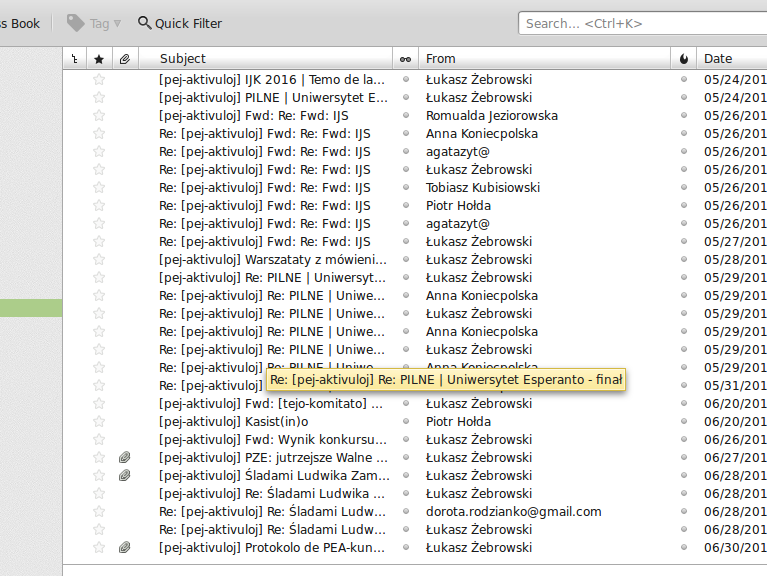
\includegraphics[scale=0.3]{ekranoj/retposhto}
	\end{center}
  \end{frame}
%%%<<<<<<<<<<<<<<<<<<<<<<<<<<<<<<<<<<<<<<<<<<<<<<<<<<<<<<<<<<<<<<<<<<<<<<<<<<<<<<<<<<<<<<<<<<<<<<
 

%%%>>>>>>>>>>>>>>>>>>>>>>>>>>>>>>>>>>>>>>>>>>>>>>>>>>>>>>>>>>>>>>>>>>>>>>>>>>>>>>>>>>>>>>>>>>>>>>
  \begin{frame}
    \frametitle{Retpoŝto}
    \framesubtitle{Ĉu vi ŝatas ĝin uzi por esperantaj projektoj?}
    \begin{itemize}
    	\item Kiom da retadresoj vi uzas?
    	\item Kiom da esperanto-rilataj (nepersonaj = malinteresaj) mesaĝoj vi ricevas semajne?
    	\item Kiom da el ili rilatas rekte al vi?
    	\item Ĉu vi ĉiam (iam ajn?) tuj recivinte la mesaĝon plenumas peton/taskon au prokrastetas?
    \end{itemize}
  \end{frame}
%%%<<<<<<<<<<<<<<<<<<<<<<<<<<<<<<<<<<<<<<<<<<<<<<<<<<<<<<<<<<<<<<<<<<<<<<<<<<<<<<<<<<<<<<<<<<<<<<
   
   
\subsection{Kiel solvi?}
   
%%%>>>>>>>>>>>>>>>>>>>>>>>>>>>>>>>>>>>>>>>>>>>>>>>>>>>>>>>>>>>>>>>>>>>>>>>>>>>>>>>>>>>>>>>>>>>>>>    
  \begin{frame}
    \frametitle{Taskolistoj?}

	\begin{block}{Ekzemplo}
    	\begin{center}
    	
\includegraphics[scale=0.5]{meme/to_do_list}
    	\end{center}
	\end{block}
    
    \begin{itemize}
    	\item Kiel tio helpas?
    	\item Ĉu vi ilin uzas por organizi sian ĉiutagan laboron?
    \end{itemize}
        
  \end{frame}    
%%%<<<<<<<<<<<<<<<<<<<<<<<<<<<<<<<<<<<<<<<<<<<<<<<<<<<<<<<<<<<<<<<<<<<<<<<<<<<<<<<<<<<<<<<<<<<<<<


   
%%%>>>>>>>>>>>>>>>>>>>>>>>>>>>>>>>>>>>>>>>>>>>>>>>>>>>>>>>>>>>>>>>>>>>>>>>>>>>>>>>>>>>>>>>>>>>>>>
  \begin{frame}
    \frametitle{Taskolistoj!}
    %http://www.learningcommons.uoguelph.ca/guides/time_management/html/making_task_list.html
    Ne forgesu, ke:
    \begin{itemize}
    	\item Tio helpas memori eĉ pri flankaj taskoj.
     	\item Oni povas taksi la prioritatojn = sukcesi ĝis limdatoj
        \item Malpli da prokrastado, ĉar vi havos realecan imagon kiom da laboro vere farendas.      
    \end{itemize}
  \end{frame}      
%%%<<<<<<<<<<<<<<<<<<<<<<<<<<<<<<<<<<<<<<<<<<<<<<<<<<<<<<<<<<<<<<<<<<<<<<<<<<<<<<<<<<<<<<<<<<<<<<


\subsection{Trello}
   
%%%>>>>>>>>>>>>>>>>>>>>>>>>>>>>>>>>>>>>>>>>>>>>>>>>>>>>>>>>>>>>>>>>>>>>>>>>>>>>>>>>>>>>>>>>>>>>>>
  \begin{frame}
    \frametitle{Mia propono: Trello.com}
    \begin{center}
    	
\includegraphics[scale=0.4]{bildoj/trello}
    \end{center}    
  \end{frame}
%%%<<<<<<<<<<<<<<<<<<<<<<<<<<<<<<<<<<<<<<<<<<<<<<<<<<<<<<<<<<<<<<<<<<<<<<<<<<<<<<<<<<<<<<<<<<<<<<
  
%%%>>>>>>>>>>>>>>>>>>>>>>>>>>>>>>>>>>>>>>>>>>>>>>>>>>>>>>>>>>>>>>>>>>>>>>>>>>>>>>>>>>>>>>>>>>>>>>
  \begin{frame}
    \frametitle{Kial -- la bildoj sinesprimas.}
    \framesubtitle{Elektu!}
    
	\begin{columns}
    \column{0.5\textwidth}
	    \begin{center}
    		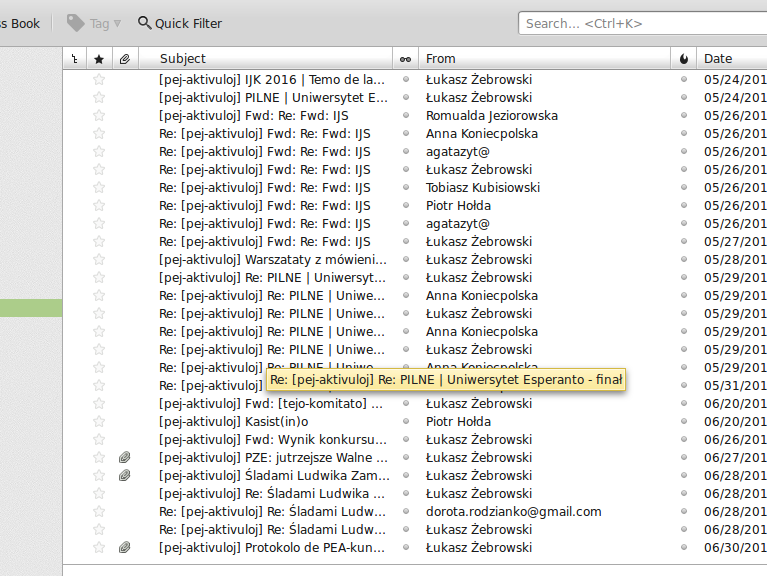
\includegraphics[scale=0.2]{ekranoj/retposhto}
    	\end{center}
	\column{0.5\textwidth}
    	\begin{center}
    	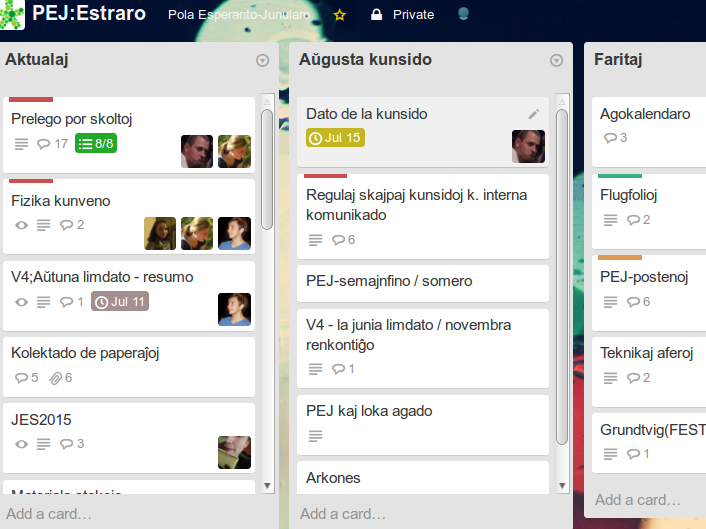
\includegraphics[scale=0.22]{ekranoj/trello-bonas-estraro}
    	\end{center}

	\end{columns}
  \end{frame}
%%%<<<<<<<<<<<<<<<<<<<<<<<<<<<<<<<<<<<<<<<<<<<<<<<<<<<<<<<<<<<<<<<<<<<<<<<<<<<<<<<<<<<<<<<<<<<<<<



%%%>>>>>>>>>>>>>>>>>>>>>>>>>>>>>>>>>>>>>>>>>>>>>>>>>>>>>>>>>>>>>>>>>>>>>>>>>>>>>>>>>>>>>>>>>>>>>>
  \begin{frame}
    \frametitle{Trello - kiu ĝin uzas?}
    
    \begin{itemize}
    	\item programistoj (kompreneble),
    	\item komercistoj por kunlabori,
    	\item sciencistoj por masturmi siajn esplorojn,
    	\item instruistoj por komuniki kun lernantoj,
    	\item verkisto por organizi verkadon de la libro
    	\item Junulara E-Semajno organizantoj.
    \end{itemize}
    
  \end{frame}
%%%<<<<<<<<<<<<<<<<<<<<<<<<<<<<<<<<<<<<<<<<<<<<<<<<<<<<<<<<<<<<<<<<<<<<<<<<<<<<<<<<<<<<<<<<<<<<<<
  
  

%%%>>>>>>>>>>>>>>>>>>>>>>>>>>>>>>>>>>>>>>>>>>>>>>>>>>>>>>>>>>>>>>>>>>>>>>>>>>>>>>>>>>>>>>>>>>>>>>
  \begin{frame}
    \frametitle{Ne nur Trello}
    \frametitle{Ekzistaj multaj similaj sistemoj!}
    
    	\begin{itemize}
    		\item \textbf{Asana}: pagenda, pli riĉa = komplika. Iam, se trello jam estos malsufiĉa...
    		\item \textbf{basecamp}: miaopinie maltaŭga por e-organizoj. 
    	\end{itemize}
  \end{frame}
%%%<<<<<<<<<<<<<<<<<<<<<<<<<<<<<<<<<<<<<<<<<<<<<<<<<<<<<<<<<<<<<<<<<<<<<<<<<<<<<<<<<<<<<<<<<<<<<<

